Consider the following feedback system:
\begin{center}
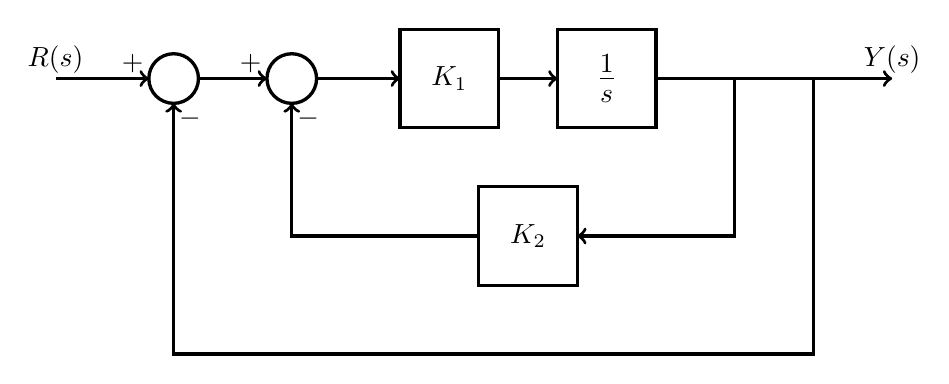
\begin{tikzpicture}[scale=1,inner sep=0pt,outer sep=0pt,very thick,
sysblock/.style={draw,rectangle,inner sep=2pt,minimum width=1.25cm,minimum height=1.25cm,very thick}]
\draw (1.5,0) node[draw,circle] (sum1) {$\rule{0pt}{18pt}$};
\draw (3,0) node[draw,circle] (sum2) {$\rule{0pt}{18pt}$};
\draw (5,0) node[sysblock] (G) {$K_{1}$};
\draw (7,0) node[sysblock] (G2) {\Large $\frac{1}{s}$};
\draw (6,-2) node[sysblock] (G3) {$K_{2}$};
\draw[->] (0,0) node[above=2pt] {$R(s)$} -- (sum1.180) node[above left=2pt] {$+$};
\draw[->] (sum1.0) -- (sum2.180) node[above left=2pt] {$+$};
\draw[->] (sum2.0) --  (G);
\draw[->] (G.0) --  (G2.180);
\draw[->] (G2.0) -- ++(1,0) |- (G3.0);
\draw[->] (G3.180) -| (sum2.-90) node[below right=2pt] {$-$};
\draw[->] (G2.0) -- ++(3,0) node[above=2pt] {$Y(s)$};
\draw[->] (G2.0) ++(2,0) -- ++(0,-3.5) -| (sum1.-90) node[below right=2pt] {$-$};
\end{tikzpicture}
\end{center}
Find $K_{1}$ and $K_{2}$ such that for a unit step input ($r(t)=u(t)$) the final value of the output $y(t)$ is  0.9 and the 1\% settling time is 5 seconds. 
Hint: find $\frac{Y(s)}{R(s)}$, and from this $K$, and either $\sigma$ or $\zeta$ and $\omega_{n}$ in terms of $K_{1}$ and $K_{2}$. 


